\documentclass[10pt,a4paper]{article}

\usepackage[margin=0.85in]{geometry}
\usepackage[T1]{fontenc}
\usepackage{lmodern}
\usepackage{microtype}
\usepackage{graphicx}
\usepackage{booktabs}
\usepackage{enumitem}
\usepackage{hyperref}
\usepackage{xcolor}
\usepackage{tikz}
\usetikzlibrary{arrows.meta, positioning, fit, backgrounds, shapes.geometric}

\hypersetup{
  colorlinks=true,
  linkcolor=blue!60!black,
  urlcolor=blue!60!black,
}

\setlist{nosep, leftmargin=*}
\setlength{\parskip}{0.35em}
\setlength{\parindent}{0pt}

\title{\textbf{Scrutinize}\\[0.3em]
\large Multi-Modal AI Embedding \& Retrieval System\\[0.2em]
\normalsize Architecture \& Project Guide}
\author{}
\date{}

\begin{document}
\maketitle
\vspace{-1.5em}

% ---------------------------------------------------------------------------
\section{Overview}

\textbf{Scrutinize} is a unified ingestion and retrieval system that lets users upload \textbf{text, audio, and video} files and later search across all modalities with a single natural-language query. A user might ask \emph{``Find the video where someone drinks milk''} and receive a cited answer pointing to the exact timestamp in an indexed video---or match a lyric in an audio file, or a passage in a PDF.

The system follows a classic \textbf{Agentic RAG} pattern: raw files are processed asynchronously into searchable \emph{segments} (text chunks with optional timestamps), stored as vector embeddings in Qdrant, and queried through a two-agent pipeline (router $\rightarrow$ retrieval $\rightarrow$ synthesis) that returns human-readable, source-cited answers.

% ---------------------------------------------------------------------------
\section{High-Level Architecture}

Four layers compose the system; a thin agent layer sits on top at query time.

\begin{center}
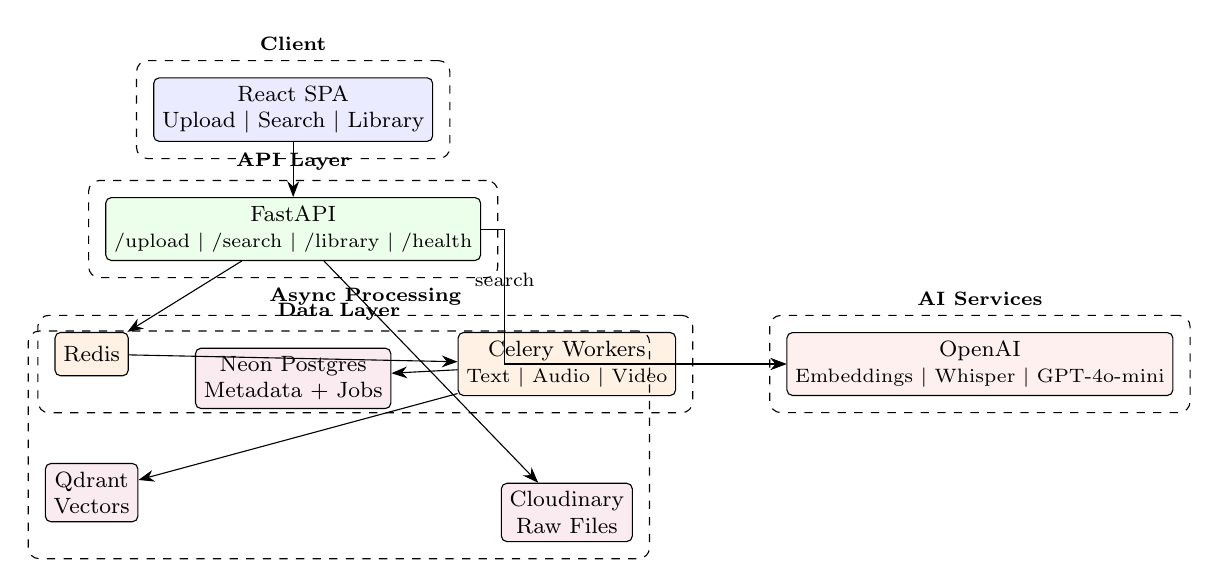
\begin{tikzpicture}[
  node distance=0.45cm and 0.6cm,
  box/.style={draw, rounded corners=2pt, align=center, font=\footnotesize,
              minimum height=0.55cm, inner sep=3pt},
  layer/.style={draw, dashed, rounded corners=4pt, inner sep=6pt},
  arr/.style={-{Stealth[length=2mm]}, font=\scriptsize}
]
  % Client
  \node[box, fill=blue!8] (fe) {React SPA\\Upload \textbar\ Search \textbar\ Library};
  \node[layer, fit=(fe), label={[font=\scriptsize\bfseries]above:Client}] (client) {};

  % API
  \node[box, fill=green!8, below=0.7cm of fe] (api) {FastAPI\\{\scriptsize /upload \textbar\ /search \textbar\ /library \textbar\ /health}};
  \node[layer, fit=(api), label={[font=\scriptsize\bfseries]above:API Layer}] (apilayer) {};

  % Queue + Workers
  \node[box, fill=orange!10, below left=0.9cm and -0.3cm of api] (redis) {Redis};
  \node[box, fill=orange!10, below right=0.9cm and -0.3cm of api] (celery) {Celery Workers\\{\scriptsize Text \textbar\ Audio \textbar\ Video}};
  \node[layer, fit=(redis)(celery), label={[font=\scriptsize\bfseries]above:Async Processing}] (queue) {};

  % Data
  \node[box, fill=purple!8, below=1.1cm of redis] (qdrant) {Qdrant\\Vectors};
  \node[box, fill=purple!8, below=1.1cm of api] (neon) {Neon Postgres\\Metadata + Jobs};
  \node[box, fill=purple!8, below=1.1cm of celery] (cloud) {Cloudinary\\Raw Files};
  \node[layer, fit=(qdrant)(neon)(cloud), label={[font=\scriptsize\bfseries]above:Data Layer}] (data) {};

  % AI (side)
  \node[box, fill=red!6, right=1.4cm of celery] (ai) {OpenAI\\{\scriptsize Embeddings \textbar\ Whisper \textbar\ GPT-4o-mini}};
  \node[layer, fit=(ai), label={[font=\scriptsize\bfseries]above:AI Services}] (ailayer) {};

  % Arrows
  \draw[arr] (fe) -- (api);
  \draw[arr] (api) -- (redis);
  \draw[arr] (redis) -- (celery);
  \draw[arr] (celery) -- (qdrant);
  \draw[arr] (celery) -- (neon);
  \draw[arr] (api) -- (cloud);
  \draw[arr] (celery) -- (ai);
  \draw[arr] (api.east) -- ++(0.3,0) |- (ai.west)
    node[pos=0.25, above, font=\scriptsize] {search};
\end{tikzpicture}
\end{center}

\textbf{Ingestion flow:} the frontend uploads a file to \texttt{/upload}. FastAPI stores the raw binary in Cloudinary, creates \texttt{files} and \texttt{processing\_jobs} rows in Neon, and enqueues a Celery task. The appropriate worker (text/audio/video) transcribes, captions, chunks, embeds, and upserts segments into Qdrant while mirroring metadata in Postgres.

\textbf{Search flow:} the user submits a query to \texttt{/search}. A \textbf{Router Agent} (GPT-4o-mini) decides modality filters and rewrites the query. The rewritten text is embedded, Qdrant returns top-$k$ segments, and a \textbf{Synthesis Agent} produces a cited natural-language answer plus structured source cards for the UI (text snippets, audio/video players with seek).

% ---------------------------------------------------------------------------
\section{Technology Stack}

\begin{table}[h]
\centering\small
\begin{tabular}{@{}lll@{}}
\toprule
\textbf{Layer} & \textbf{Technology} & \textbf{Role} \\
\midrule
Frontend & React, Vite, Tailwind & Chat-style UI, upload, library browser \\
API & FastAPI, SQLModel, Pydantic & REST endpoints, validation, OpenAPI docs \\
Queue & Redis + Celery & Background media processing \\
Vector DB & Qdrant & Similarity search with payload filters \\
Relational DB & Neon (Postgres) & Files, jobs, segments (source of truth) \\
Object Storage & Cloudinary & CDN-backed raw file URLs for playback \\
AI & OpenAI API & Embeddings, Whisper, vision captioning, agents \\
Media & FFmpeg & Audio extraction, keyframe sampling from video \\
\bottomrule
\end{tabular}
\end{table}

\textbf{Embedding strategy (MVP):} all modalities are converted to \textbf{text} (transcripts, captions, chunks) and embedded with \texttt{text-embedding-3-small} (1536-dim) into a single Qdrant collection. This enables cross-modal search in one vector space. A planned Phase~2 adds named vectors (CLIP visual, CLAP audio) per Qdrant point for native visual/acoustic similarity.

% ---------------------------------------------------------------------------
\newpage
\section{Ingestion Pipelines}

\textbf{Text} --- Upload $\rightarrow$ Cloudinary $\rightarrow$ extract \& chunk ($\sim$300--500 tokens) $\rightarrow$ embed $\rightarrow$ Qdrant + Neon.

\textbf{Audio} --- Upload $\rightarrow$ Cloudinary $\rightarrow$ Whisper transcription (timestamped) $\rightarrow$ segment into 15--30\,s windows $\rightarrow$ embed $\rightarrow$ Qdrant + Neon.

\textbf{Video} --- Upload $\rightarrow$ Cloudinary $\rightarrow$ FFmpeg extracts audio track \emph{and} keyframes $\rightarrow$ Whisper transcribes audio, GPT-4o-mini captions frames $\rightarrow$ merge into time-aligned segments $\rightarrow$ embed $\rightarrow$ Qdrant + Neon.

Each segment stored in Qdrant carries payload fields: \texttt{modality}, \texttt{content}, \texttt{file\_id}, \texttt{start\_time}/\texttt{end\_time}, \texttt{source\_path}, and \texttt{title}.

% ---------------------------------------------------------------------------
\section{API Endpoints}

\begin{table}[h]
\centering\small
\begin{tabular}{@{}llp{5.5cm}@{}}
\toprule
\textbf{Method} & \textbf{Path} & \textbf{Purpose} \\
\midrule
POST & \texttt{/upload} & Accept file; store in Cloudinary; enqueue processing job \\
GET  & \texttt{/status/\{job\_id\}} & Poll job progress (pending $\rightarrow$ indexed/failed) \\
POST & \texttt{/search} & Natural-language query $\rightarrow$ cited answer + sources \\
GET  & \texttt{/library} & Browse indexed files and their segments \\
GET  & \texttt{/health} & Dependency health (Neon, Redis, Qdrant, Cloudinary) \\
\bottomrule
\end{tabular}
\end{table}

Rate limiting middleware protects upload and search endpoints. API keys (OpenAI, Cloudinary, Neon) remain server-side only; the frontend communicates exclusively with FastAPI.

% ---------------------------------------------------------------------------
\section{Project Structure}

\begin{verbatim}
Scrutinize/
  frontend/          React + Vite SPA (src/components, api/)
  backend/
    app/
      api/           upload, search, library routes
      services/      processors, embedding, vector store, agents
      workers/       Celery tasks (process_text/audio/video)
      models/        SQLModel ORM (File, Segment, ProcessingJob)
      middleware/    rate limiting
    migrations/      Neon schema SQL
  tests/             unit, integration, system, security tiers
  docs/              architecture, modules, runbooks
  deploy/fly/        Fly.io deployment configs
  docker-compose.yml Redis, Qdrant, backend, worker
\end{verbatim}

% ---------------------------------------------------------------------------
\section{Getting Started}

\textbf{Prerequisites:} Neon Postgres (pooled connection string), Cloudinary account, OpenAI API key, Docker.

\begin{enumerate}
  \item Copy \texttt{.env.example} to \texttt{backend/.env} and fill in \texttt{DATABASE\_URL}, \texttt{CLOUDINARY\_*}, \texttt{OPENAI\_API\_KEY}.
  \item Apply schema: \texttt{make install-backend \&\& make db-migrate}
  \item Start backend stack: \texttt{docker compose up --build} (Redis, Qdrant, API, Celery worker)
  \item Start frontend: \texttt{make install-frontend \&\& make frontend-dev}
  \item Open \url{http://localhost:5173} (frontend) and \url{http://localhost:8000/docs} (API)
\end{enumerate}

The frontend displays a green \textbf{API connected} badge when \texttt{/health} reports all dependencies are reachable.

\textbf{Testing:} \texttt{make test-unit}, \texttt{make test-integration}. CI (GitHub Actions) runs unit, integration, system, and security tiers on every push to \texttt{main}.

\textbf{Deployment:} production configs live under \texttt{deploy/fly/} for Fly.io (API, worker, Redis, Qdrant). See \texttt{docs/runbooks/fly-io-deploy.md} for the full runbook.

% ---------------------------------------------------------------------------
\section{Design Decisions}

\begin{itemize}
  \item \textbf{FastAPI over Node gateway} --- the ML/media stack (Whisper, FFmpeg, OpenAI SDK) is Python-first; a single-language backend avoids microservice overhead.
  \item \textbf{Qdrant over pgvector} --- native vector DB with rich payload filtering and future multi-vector support per point.
  \item \textbf{Neon + Cloudinary split} --- Postgres handles relational queries (jobs, joins, pagination); Cloudinary serves playable media URLs with CDN delivery.
  \item \textbf{Celery over BackgroundTasks} --- video ingestion (frame extraction + multiple API calls) exceeds HTTP timeouts; workers scale horizontally.
  \item \textbf{Two-agent RAG} --- Router Agent handles query understanding and modality filtering; Synthesis Agent produces cited answers. Minimal agent count, production-grade pattern.
\end{itemize}

\end{document}
